%by Elena C. WORK IN PROGRESS
\subsection{Leapfrog Algorithm}
The Velocity Verlet algorithm shown previously (Algorithm \ref{alg:velocity_verlet}) can be modified to reduce the computational cost.\\ In particular, compute a force is quite expensive: computing the force twice will require twice the simulation time. One solution to reduce the computational cost is to merge the momenta shifts together (using the same value of the force): this leads to a slightly faster simulation, but on the other side this kills the possibility of printing the values of p and q at the same time (access to the phase space). This solution is called \textbf{Leapfrog algorithm}.\\
\begin{algorithm}[H]
			\caption{Leapfrog algorithm}
			\label{alg:leapfrog}
			\begin{algorithmic}[1]
			    \State $p=p+f*\Delta t/2$	\For{$i=1,...,nsteps$}
    			\State	$q=q+p/m \Delta t$
                 \State	$f=force(q)$
    			\State	$p=p+f*\Delta t$
				\EndFor
			\end{algorithmic}
		\end{algorithm}
Momentum and position are moved in an alternate way: at the end of a cycle, we do not find the values of the positions and momenta at the same timestep, they are found at a difference of half timestep. Slightly faster than Velocity Verlet, not very significant. 
\begin{figure}[H]
    \centering
    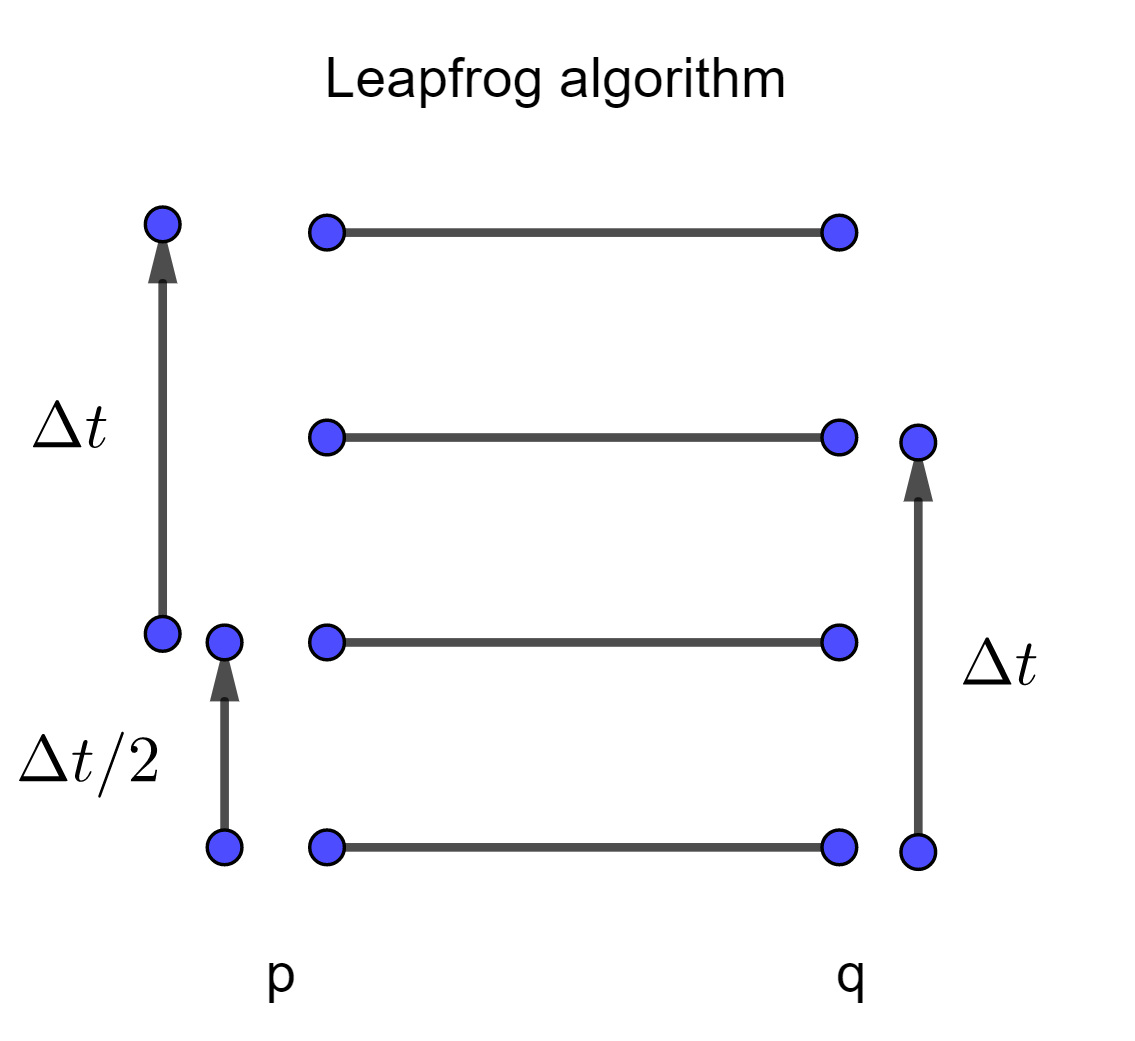
\includegraphics[width=50mm,scale=0.5]{Integrators/images/leapfrog.png}
    \caption{Scheme of the leapfrog algorithm}
    \label{fig:leapfrog}
\end{figure}
\subsection{Position Verlet}
Another alternative to the Velocity Verlet algorithm it is the so-called \textbf{Position Verlet algorithm}.
\begin{algorithm}[H]
			\caption{Position Verlet}
			\label{alg:position_verlet}
			\begin{algorithmic}[1]
        	\For{$i=1,...,nsteps$}
			\State	$q=q+p/m* \Delta t/2$
			\State	$f=force(q)$
			\State	$p=p+f*\Delta t$
			\State	$q=q+p/m* \Delta t/2$
				\EndFor
			\end{algorithmic}
		\end{algorithm}
This algorithm is the swapped version of Velocity Verlet, where the free particle is evolved for half timestep, then the infinite mass system is evolved for one timestep, then the free particle again for half timestep. 
\begin{itemize}
    \item \textbf{Advantages:} the force is computed only once, which is computationally advantageous (only one update of the momentum).
    \item \textbf{Disadvantages:} I cannot print the total energy. Potential energy needs to be computed with a similar procedure to the computation of forces (very expensive). Therefore, it is more convenient to compute forces and energies at the same time, but it is not possible with Position Verlet. Moreover, this algorithm is less used than Velocity Verlet, which is the simplest one.
\end{itemize}

\subsection{Other considerations on the Velocity Verlet algorithm}
Let us recall the Velocity Verlet algorithm:
    \begin{equation}\label{velocityverlet}
            \begin{cases}
                q(t+\Delta t)= q(t)+\frac{p(t)}{m}\Delta t+ \frac{f(t)}{m}\frac{\Delta t^2}{2}\\
                p(t+\Delta t)= p(t)+\frac{f(t)}{2}\Delta t+ \frac{f(t+\Delta t)}{2}\Delta t
            \end{cases}
            \end{equation}
Let's prove that the trajectories obtained with Velocity Verlet are equivalent to those obtained with Verlet algorithm. Trajectories are exactly time reversible, which means that we are allowed to compute $q(t-\Delta t)$ changing the sign of $\Delta t$ in the first equation \ref{velocityverlet}:
\begin{equation}\label{t-dt}
q(t-\Delta t)= q(t)-\frac{p(t)}{m}\Delta t+ \frac{f(t)}{m}\frac{\Delta t^2}{2}
\end{equation}
Let us sum $q(t-\Delta t)$ and $q(t+\Delta t)$ (first eq. \ref{velocityverlet} and eq. \ref{t-dt}):
\begin{equation*}
    q(t-\Delta t)+q(t+\Delta t)=2q(t)+\frac{f(t)}{m}\Delta t^2
\end{equation*}
This is consistent because equation \ref{velocityverlet} for the positions resembles a Taylor expansion of q.  The introduction of operator formalism is significant only for the sake of studying the evolution of momenta, while the evolution of positions is equivalent to the one obtained with the Verlet algorithm. 
In fact, the same trajectory results from the application of Verlet and Velocity Verlet algorithms.\\
Differences between the two algorithms are found by the fact that the Verlet algorithm considers differences between positions (current position $q(t_0)$ minus previous position $q(t_0-\Delta t$)): this leads to large round-off errors. Meanwhile, this problem is not present in Velocity Verlet, which is more numerically stable. Moreover, Velocity Verlet already includes a definition of the velocity, not present in Verlet algorithm: in the former case it is possible to compute the total energy and check if it is conserved.
We recall the properties of Velocity Verlet already discussed in section \ref{chapt:properites_vel_verlet}:
\begin{itemize}
\item \textbf{Trajectory is time reversible.}
\item \textbf{Volume in phase space is conserved.}
\item \textbf{Energy is not conserved}
\end{itemize}
Let us check the latter property for a simple example.
\subsubsection{Harmonic oscillator}
Force is given by 
\begin{equation*}
    f=- k q
\end{equation*}
Change slightly the notation:
\begin{equation*}
    \begin{cases}
        q=q(t)\\
        q'=q(t+\Delta t)
    \end{cases}
\end{equation*}
\begin{equation*}
    \begin{cases}
        q'=q+\frac{p}{m}\Delta t -\frac{k}{m}\frac{q \Delta t^2}{2}=(1-\frac{k}{m}\frac{\Delta t^2}{2})q+\frac{\Delta t}{m}p\\
        p'=p-\frac{k q \Delta t}{2}-\frac{k q' \Delta t}{2}
    \end{cases}
\end{equation*}
Substituting the first equation into the second equation we obtain:
\begin{equation}
    p'=p-k q \Delta t-\frac{k p \Delta t^2}{2m}+\frac{k \Delta t^3 k q}{4 m} = (1-\frac{k}{2m}\Delta t^2)p+(-k \Delta t+\frac{k^2 \Delta t^3}{4 m})q
\end{equation}
In a matrix form:\\
\begin{equation}
  \begin{pmatrix}
    q'\\
    p'
  \end{pmatrix}
  =
  \begin{pmatrix}
    1-\frac{k}{m}\frac{\Delta t^2}{2} & \frac{\Delta t}{m} \\
    -k \Delta t+\frac{k^2 \Delta t^3}{4 m} & 1-\frac{k}{m}\frac{\Delta t^2}{2}
  \end{pmatrix} 
  \begin{pmatrix}
    q \\
    p
  \end{pmatrix}
\end{equation}
  If k=m=1 (unit-less expression):
\begin{equation}
  \begin{pmatrix}
    q'\\
    p'
  \end{pmatrix}
  =
  \begin{pmatrix}
    1-\frac{\Delta t^2}{2} & \Delta t \\
    -\Delta t+\frac{\Delta t^3}{4} & 1-\frac{\Delta t^2}{2}
  \end{pmatrix} 
  \begin{pmatrix}
    q \\
    p
  \end{pmatrix}
\end{equation}
If energy is conserved, the exact solution should be given by a circular trajectory. In other words, the energy conservation is satisfied if the transformation matrix is a rotation.
A rotation matrix is given by
\begin{equation}
A=
    \begin{pmatrix}
      \cos{\theta} & -\sin{\theta} \\
      \sin{\theta} & \cos{\theta}
    \end{pmatrix}
\end{equation}
Therefore, we could impose $\cos{\theta}=1-\frac{\Delta t^2}{2}$ and it is okay because the elements on the diagonal are equal, but $ \Delta t\neq -(-\Delta t+\frac{\Delta t^3}{4})$ in general. Let us also check if the determinant is equal to 1 as the determinant of a rotational matrix.
\begin{equation}
    det(A)= \left(1-\frac{\Delta t^2}{2}\right)^2-\left(-\Delta t+\frac{\Delta t^3}{4}\right)*\Delta t =1
\end{equation}
Still, this is not exactly a rotational matrix but only approximately. This implies that, starting from a point on the trajectory, the next one will not follow the exact trajectory. In order to study the behaviour of the trajectory, i.e., if the trajectory explodes, implodes or fluctuates, let us consider the eigenvalues of $A$.
\begin{equation}
det(A-\lambda \mathbb{1})=(1-\frac{\Delta t^2}{2}-\lambda)^2-(-\Delta t+\frac{\Delta t^3}{4})*\Delta t=0
\end{equation}
\begin{equation*}
(1-\frac{\Delta t^2}{2}-\lambda)^2=(-\Delta t+\frac{\Delta t^3}{4})*\Delta t
\end{equation*}
\begin{equation*}
    \lambda_{1,2}=1-\frac{\Delta t^2}{2}\pm \sqrt{-\Delta t^2 + \frac{\Delta t^4}{4}} 
\end{equation*}
Eigenvalues can be either both real or both complex and conjugated (see graph \ref{fig:complexplane}) in the former case, their product should be 1 ($\lambda_1*\lambda_2=1$). 
\begin{figure}[H]
    \centering
    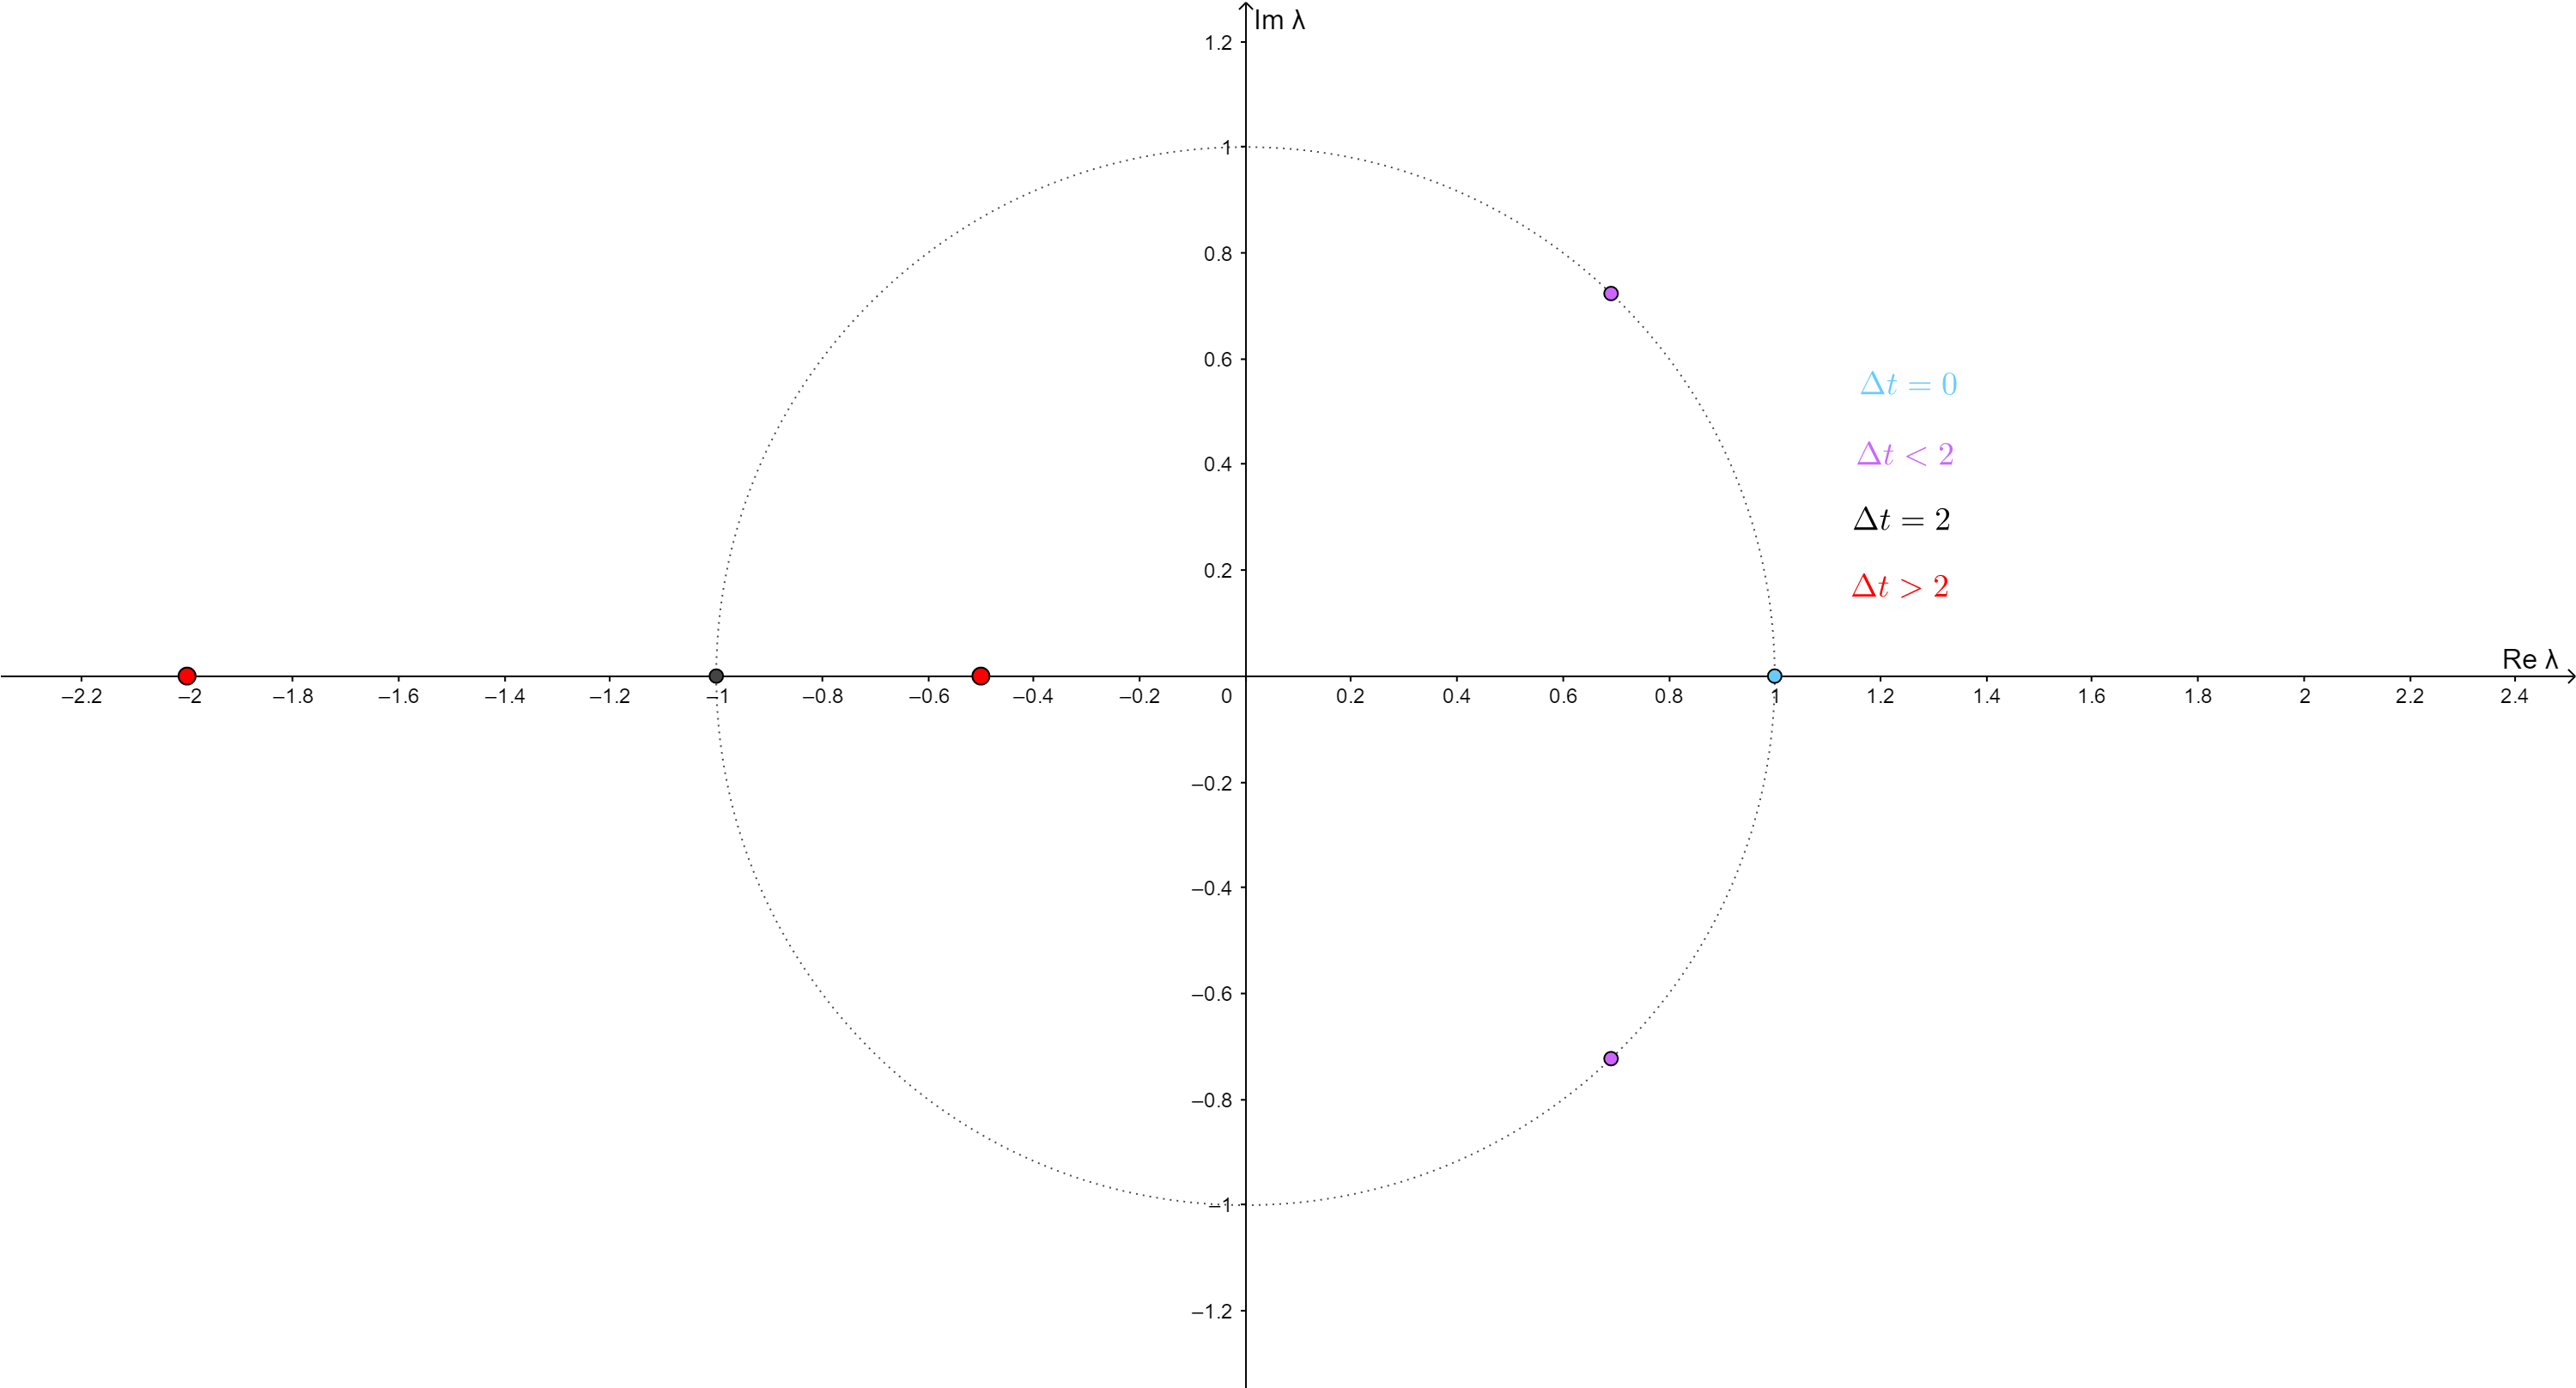
\includegraphics[scale=3.0]{Integrators/images/complexplane.png}
    \caption{Possible eigenvalues of the matrix $A$}
    \label{fig:complexplane}
\end{figure}
In the case where they are complex, their imaginary part is opposite and the real parts are equal.
After n steps:
\begin{equation}
    \begin{pmatrix}
      q' \\
      p'
    \end{pmatrix}
    = A^n
    \begin{pmatrix}
      q \\
      p
    \end{pmatrix}
\end{equation}
Check the behaviour for a large number of time steps ($n\xrightarrow{}\infty$):
\begin{itemize}
    \item if $A^n$ contains some infinite term, then the trajectory will diverge.
    \item if $A^n$ goes to 0, then the trajectory will converge (oscillate around the circular trajectory).
\end{itemize}
The eigenvalues of $A^n$ are equal to the eigenvalues of $A$ raised to the n-th power, therefore:
\begin{itemize}
    \item  $\lambda_1=\lambda_2=-1$: trajectory will oscillate\footnote{$\lambda_1=\lambda_2=1$ is the case when the timestep is equal to zero, therefore the system is not moving}. $$\Delta t = 2$$
    \item $\lambda_1> -1$, $\lambda_2< -1$ or $\lambda_2> -1$, $\lambda_1< -1$: matrix explodes, trajectory diverges. $$\Delta t > 2$$
    \item complex eigenvalues with unitary modulus: trajectory will oscillate.  $$\Delta t < 2$$
\end{itemize}
Threshold for stability of a numerical simulation:
\begin{equation}
    \Delta t < \frac{T}{\pi}
\end{equation}
This is the theoretical limit for the timestep, given the period. The criterion for the timestep is the same for Verlet and Velocity Verlet.
\subsection{Multiple springs}
Let us consider a situation where there are 3 particles with the same mass connected by springs with $k_1 >> k_2$. Let us estimate the maximum time step that should be used. The solution is to take the stiffest spring to impose the limit on the timestep, i.e., that gives the shortest timestep.
In general, this condition is given by the fastest degree of freedom, in other words, by the lightest possible atom with the stiffest spring. This is the way to find the upper bound for our timestep:
computing the period $2\pi \sqrt{\frac{m}{k}}$.
If energy is sufficiently conserved, this means that the timestep is small enough. It is difficult to predict a priori a good value of the timestep because there could be nonlinear potentials.

